% 126-63(126쪽) — 점 P 의 속도 v(t) 의 그래프(0 ≤ t ≤ 7 · 꺾은선). 스캔 화질이 낮아 TikZ 로 다시 그림.
% 원문에 있는 것만: 꺾은점 (0,0)-(1,1)-(4,-2)-(5,1)-(6,1)-(7,0) · 라벨 v(t) · t · O · t 눈금 1 2 4 5 6 7 · v 눈금 1 과 -2 · 안내 파선.
% 2 와 4 는 원문처럼 t축 위, 1 · 5 · 6 · 7 은 t축 아래에 적는다. 그 밖의 눈금·수치는 넣지 않는다.
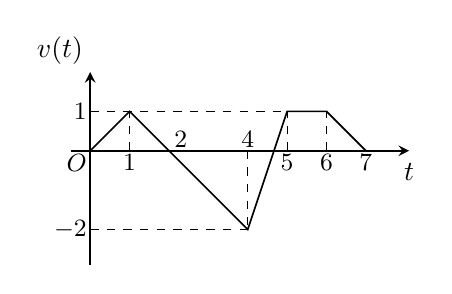
\begin{tikzpicture}[x=0.50cm, y=0.50cm, line width=0.5pt,
  tick/.style={font=\small, inner sep=1pt}]
  \draw[->, >=stealth, line width=0.7pt] (-0.5,0) -- (8.1,0) node[below=1pt] {$t$};
  \draw[->, >=stealth, line width=0.7pt] (0,-2.9) -- (0,2.0) node[above left=-1pt] {$v(t)$};
  \node[tick, below left] at (0,0) {$\pt{O}$};
  % 안내 파선(원문)
  \draw[dashed, line width=0.35pt] (0,1) -- (5,1);
  \draw[dashed, line width=0.35pt] (0,-2) -- (4,-2);
  \draw[dashed, line width=0.35pt] (1,0) -- (1,1);
  \draw[dashed, line width=0.35pt] (4,0) -- (4,-2);
  \draw[dashed, line width=0.35pt] (5,0) -- (5,1);
  \draw[dashed, line width=0.35pt] (6,0) -- (6,1);
  % 그래프
  \draw[line width=0.6pt] (0,0) -- (1,1) -- (4,-2) -- (5,1) -- (6,1) -- (7,0);
  \node[tick, below] at (1,0) {$1$};
  \node[tick, above] at (2.3,0) {$2$};
  \node[tick, above] at (4,0) {$4$};
  \node[tick, below] at (5,0) {$5$};
  \node[tick, below] at (6,0) {$6$};
  \node[tick, below] at (7,0) {$7$};
  \node[tick, left] at (0,1) {$1$};
  \node[tick, left] at (0,-2) {$-2$};
\end{tikzpicture}
